\chapter{Background, Motivation, and Overview}
\label{chap:intro}

%=====================================================================================================
\section{Introduction}
\label{intro}
%About 5 pages answering questions 1 and 2 above, along with describing the broad research area. This section provides the reader with enough information to understand and appreciate the thesis statement. This includes giving the motivation for the research, defining terms and formulating the problem. Often, subsections labeled ``Background'' and ''Motivation'' will be included in this section. This section typically provides answers to the questions ``What problem do you want to solve'' and ''Who cares about this problem and why?'' The Background subsection could contain the discussion about the broader research area.

%===================================================
\subsection{Problem Motivation}
\label{motivation}

Because of rapid advancement in technology, more and more Artificial Intelligence (AI) and robotics systems are appearing in various aspects of people's lives. For example, there are systems that assist humans to schedule limousine services~\cite{Chun2010Limousine}, to evaluate and control the damage of an oil spill\footnote{http://spectrum.ieee.org/robotics/industrial-robots/the-gulf-spills-lessons-for-robotics}, to support search and rescue missions~\cite{Casper2003WTO, Lin2010Supporting}, and to provide treatment to children with autism~\cite{Robins2009From}. Such abundant and rapidly growing applications increase the set of possible interactions between human users and autonomous systems. The humans in such interactions are not likely the designers of the autonomous systems, but these humans must still manage the autonomy.

Although AI and robotics systems have grown to be able to handle increasingly complex tasks in uncertain environments, human assistance and supervision are often needed~\cite{Bainbridge1983Ironies}. Even for fully autonomous systems, human input can potentially improve the system's performance and safety. Human experts can use domain-specific knowledge to assist an AI/robotics system when it deals with changing environments, uncertainty, and case-specific scenarios. Therefore, it is necessary to design tools and interfaces that enable human users working with an AI/robotics system to manage the autonomous behaviors of the system efficiently and effectively; such tools can improve task performance and the experience of a human partner in human-automation interaction. 

However, human users often do not understand how the internal mechanisms of an autonomous system work especially when the system is complicated or when complex algorithms are involved. Instead, humans must rely on their own mental models of the system during operation~\cite{Moray1999Mental}. Supporting human interaction requires a design approach that lets users understand how autonomous behaviors can be influenced without getting deeply into how autonomy really works. This requirement makes designing for autonomy management especially challenging.

%===================================================
\subsection{General Solution Approach}

We propose that autonomy management tools should let users hierarchically manage information provided to an AI/robotics system. Good information management tools should allow users to influence the autonomous behaviors of the system at multiple scales without the need for tedious direct/manual control. This dissertation presents autonomous algorithms/components and autonomy management tools/interfaces designed at different scales and show that this approach improves the performance of the human-automation team and the experience of the human-automation interaction.

The term ``information'' here covers a wide range of things including \textit{knowledge of the environment} (including other humans, equipment, and changes in the physical surroundings), \textit{knowledge of the task} at hand (including processes, procedures, rules, past experiences, etc.), and \textit{interactions among various entities} (task, environment, human, and the system). In theory, an AI/robotics system can obtain, process, and analyze information in order to complete the desired tasks. In practice, however, the system often has limited sensing and reasoning capabilities, and there is useful information the system is either not capable of obtaining or not able to understand/process. Such information can even be produced by the system itself. Often, the human users of such systems have much better ``information sensing'' capabilities. These capabilities allow humans to obtain information from their own resources such as past experiences, domain-specific training, external communications (with team members, external systems, etc.), or even the AI/robotics system itself. The human user is also capable of ``digesting'' various information and then feeding the ``filtered'' information to the system in forms the system can understand. In a sense, the human user acts as an ``intelligent sensor'' for the system. At the same time, by deciding what information to provide to the system, the human user has a way of influencing the system's autonomous behaviors without the need for tedious manual control.

%\begin{figure}
%\centering
%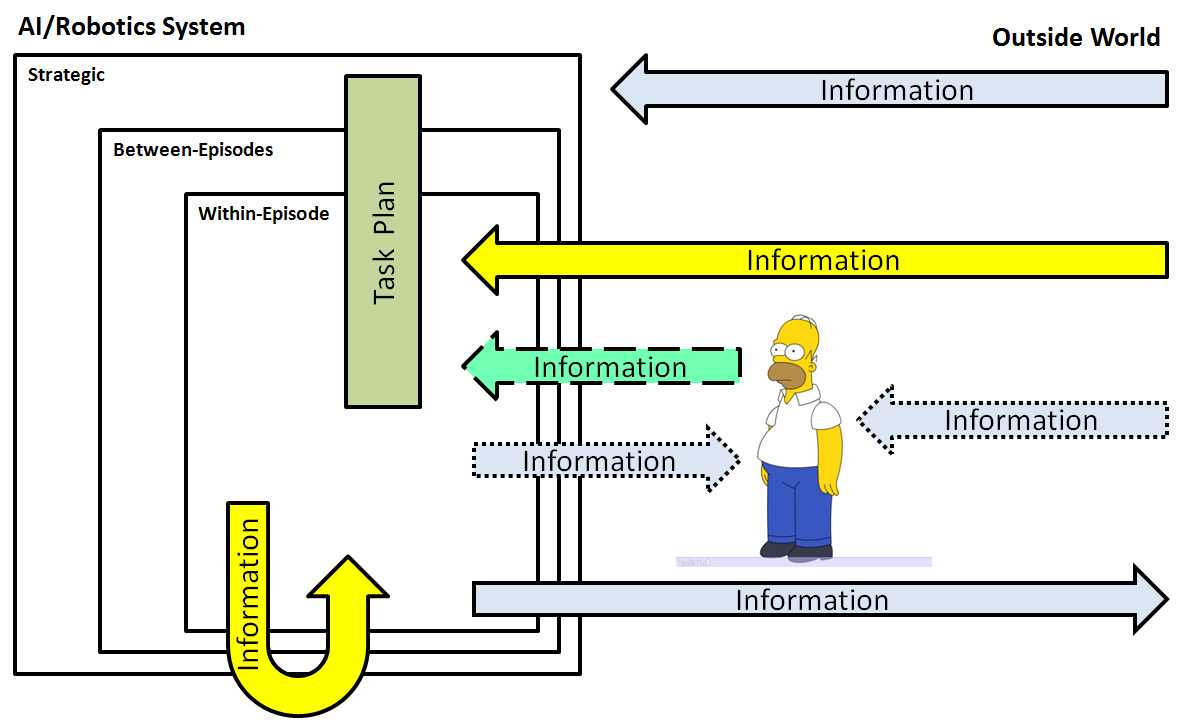
\includegraphics[width=4.5in]{System.png}
%\caption{Diagram showing relationship between the human user and the AI/robotics System with respect to information management.}
%\label{system}
%\end{figure}

%Figure~\ref{system} shows a diagram of the relationship between the human user and the AI/robotics system. The system must be capable of receiving the outside information at different scales (solid yellow arrow at the top). The system has some degree of sensor-processing, so it naturally uses internal information to make decisions (solid yellow arrow at the bottom). The human can sense and process information the system is not capable of handling. Such information can be directly from the outside world (dotted blue arrow on the right) or perceived through the system's sensors (dotted blue arrow on the left). The human processes the information and feeds filtered information to the system, in forms the system can understand (dashed green arrow), in order to influence the system's autonomous behaviors.

\begin{figure}
\centering
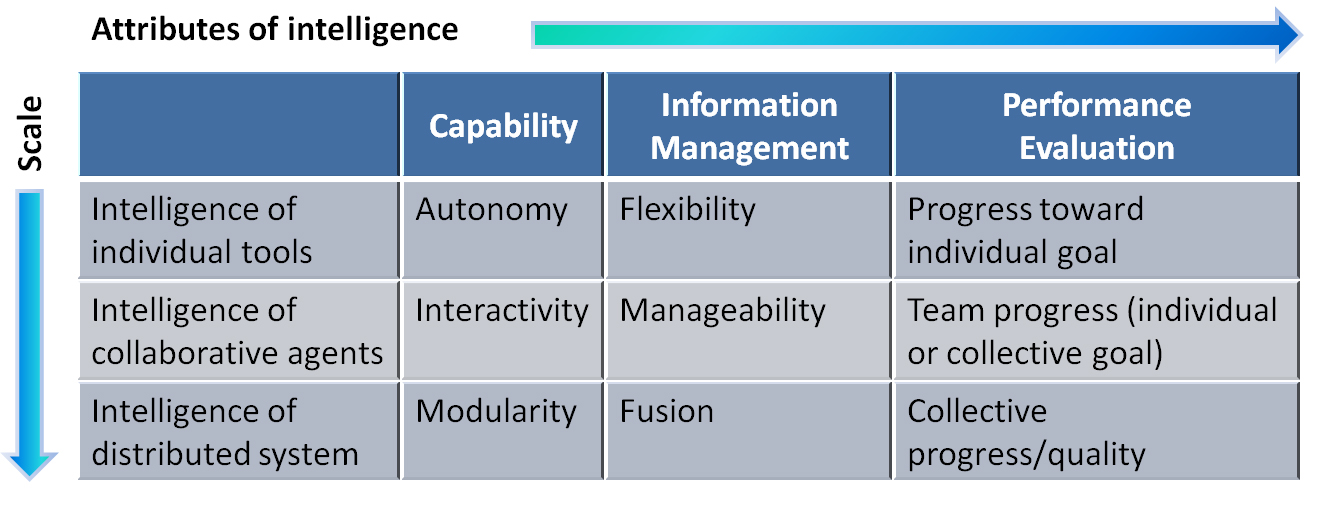
\includegraphics[width=6in]{IntegrationChallenges.JPG}
\caption{Autonomy integration challenges defined along two dimensions. Horizontal dimension: attributes of intelligence. Vertical dimension: scale.}
\label{challenges}
\end{figure}

In an overall intelligent system, autonomy typically exists as component tools with the goal to offload portions of responsibility to autonomous algorithms. Figure~\ref{challenges} lists some key elements of the autonomy integration challenges we identified in~\cite{Lin2010Supporting} along two dimensions: \textit{attributes of an intelligent system} (capability, information management, performance evaluation) and \textit{scale} (individual versus group, expanded to include a new row for intelligence of collaborative agents). This table provides guidelines on what attributes should be designed into an autonomous component when it is part of a human-automation collaboration team and a much larger distributed intelligent system. As an individual tool, the autonomous component needs to be able to perform certain tasks (\textbf{autonomy}). It should be able to work with different scenarios and can be interrupted, temporarily aborted, and possibly resumed later depending on information available to the operator (\textbf{flexibility}). If a human agent is in a collaborative team with the autonomous agent for the same task, the autonomous component must provide ways of interaction (\textbf{interactivity}) so the human can manage how the autonomous component works based on information only the human can interpretate (\textbf{manageability}). Then in order to integrate the autonomous component into the overall distributed system, the autonomous component has to be modular so it is easy for human operators to share responsibilities or (partially) take on responsibilites of different roles (\textbf{modularity}). And information from various sources (including information output from autonomous components) need to be combined and presented intelligently in an efficient way to relavant users (\textbf{fusion}). Autonomous components presented in this dessertation all display these important attributes. Specifically, we design our autonomous components with the capability to interact with information representations so the human agent can manage autonomy by hierarchically managing information. 

Good autonomy management tools will only let users manage information that allow them to develop a clear causal relationship between information management actions and the changes of the system's autonomous behaviors. Examples of such information include what data set to use to train the system and which tasks deserve more attention. Such causal relationships make developing correct mental models of the system easier leading to improved task performance. 

Information can be managed at different temporal scales. 
%We use the term ``resolution'' to describe the levels of details involved. Working at a high resolution is like working with individual pixels in an image to achieve fine precision, whereas working at a low resolution is more like working on object attributes such as shapes or shadings that are viewed better when one takes a step back from the image and ignores the fine details. Similarly, managing autonomy at a high resolution involves managing the actions of the AI/robotics system in fine details (e.g., managing waypoints a UAV should follow), and at a low resolution autonomy management might deal with strategic planning following generate trend (e.g., predicting and identifying high priority areas in a WiSAR operation).
We propose a general hierarchical framework that focuses on the following three scales: \textbf{Strategic}, \textbf{Between-Episodes}, and \textbf{Within-Episode}\footnote{The term ``episode'' we use is similar to the one Russell and Norvig define in Chapter 2 of~\cite{Russell2009Artificial} when they discussed episodic vs. sequential task environments. Our definition is more relaxed to include cases where actions taken in previous episodes might impact the current episode with respect to task objectives, but each episode is still by itself a separate and self-contained unit.}. 

When an AI/robotics system is given a task, the system can generate an initial plan based on its model(s) of how this kind of task is generally performed. This step is planning at the \textbf{Strategic} scale. Since the same task can be performed in different case scenarios (such as different environments, constraints, or phases of the operation), case-specific attributes and requirements need to be evaluated, and the initial plan needs to be tailored to the specific case. This step is planning at the \textbf{Between-Episodes} scale. During execution of the task, the plan is carried out, but as new information becomes available or when the environment changes due to uncertainty, the plan can be modified in real time to achieve better task performance. This step is planning at the \textbf{Within-Episode} scale. If the user of the system can manage information provided to the system by selecting what information to provide at what scale, he/she can change the system plan at different scales and indirectly influence the autonomous behaviors of the system.

To evaluate the usefulness of the proposed autonomy management approach, we apply it to the application domain of using an Unmanned Aerial Vehicle (UAV) to support Wilderness Search and Rescue (WiSAR).

%===================================================
\subsection{Application Domain}

A small camera-equipped UAV can quickly and cheaply provide aerial imagery of a wilderness search area, especially hard-to-reach areas~\cite{Goodrich2008Supporting}. The MAGICC lab, the HCMI lab, and the Computer Vision Lab at BYU have been researching UAV technologies for several years and made great progress in UAV path-planning control, user interface design, and computer vision~\cite{Lin2010Supporting}. Figure~\ref{SystemComponents} shows the various components developed by our research group.

\begin{figure}
\centering
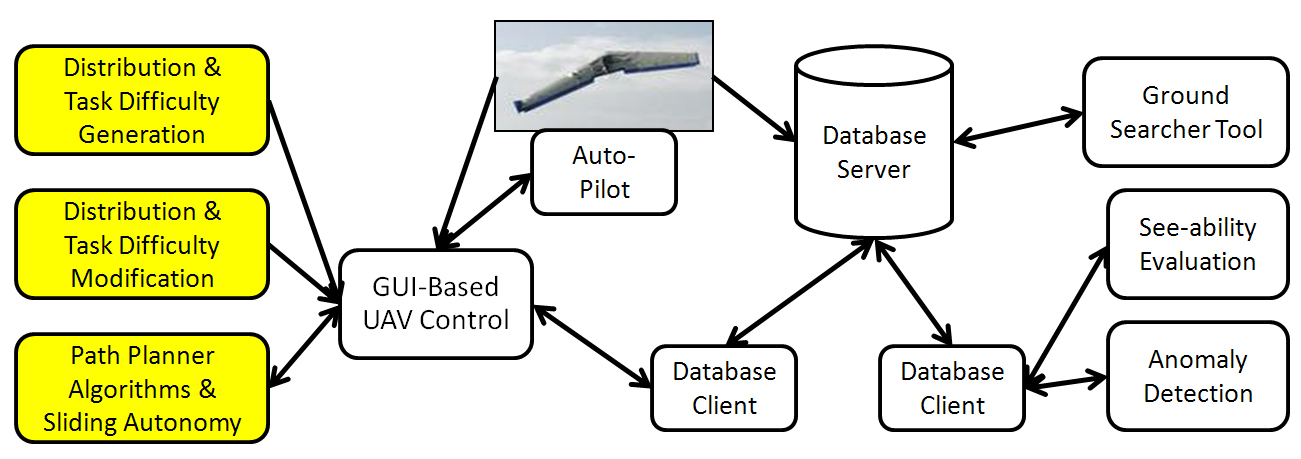
\includegraphics[width=6in]{UAVWiSARComponents.JPG}
\caption{Various components of the overall intelligent system (a distributed system) of using a UAV to support Wilderness Search and Rescue.}
\label{SystemComponents}
\end{figure}

Past UAV field trials indicate that real WiSAR searchers like not having to worry about keeping the UAV in the air or setting waypoints manually. Autonomy that offloads or complements some search work is useful, but searchers also need to be able to manage where to send the UAV as new evidence is gathered or hard-to-reach areas are identified. Ideally, searchers need not understand the statistical models or complex algorithms used by the UAV. Rather, searchers should manage autonomy by managing information provided to the UAV system at different scales. We focus on two important representations of information: a \textit{probability distribution map} and a \textit{task-difficulty map}.

At the \textbf{Strategic} scale, we have developed a Bayesian model, \textbf{TBMod}, to predict the probability distribution of the missing person's likely location. This distribution can be based on terrain features of the search area and past human behavior data in the form of GPS track logs. We propose to develop an autonomy management tool, \textbf{ParamMod}, that lets the user manage ``user-friendly'' parameters of the model with real-time feedback on how changes affect the model-generated probability distribution. At the \textbf{Between-Episodes} scale, we propose two autonomy management tools: \textbf{DistMod}, a tool that lets the user modify the probability distribution to specify areas of focus with simple gestures, and \textbf{DiffMod}, a tool that lets the user use scribbles to modify the task-difficulty map, a representation marking areas with low probability of detection. At the \textbf{Within-Episode} scale, we will extend existing path-planning algorithms to support partial detection and real-time feedback. We also propose an autonomy management tool, \textbf{SlideMod}, that lets the user manage UAV autonomy by controlling how much time is granted to a UAV flight. 


%=====================================================================================================
\section{Related Work}
\label{related}
%About 2 pages answering question 3 above. This section contains a survey of the literature directly related to the problem you are trying to solve (i.e., thesis statement) and should demonstrate to your readers that you understand the context of your work. This is a place for you to position your contribution to your specific research area relative to other work that has been done, and to state how your work builds on the previous work. In most cases there will be only a small overlap between the papers discussed in this section and the papers related to the broader research area. This section answers the question ``What have others done to solve the problem and why is this inadequate?''

In their in-depth survey paper~\cite{Goodrich2007HRISurvey}, Goodrich and Schultz define the HRI problem as ``understanding and shaping the interactions between one or more humans and one or more robots.'' They also specified robot-assisted search and rescue as a key area for HRI research. In this section we first present related work in the general research area, then discuss related research more specific to the domains of using UAVs to support Wilderness Search and Rescue.

%===================================================
\subsection{General Research Area}

%Sheridan and Verplank~\cite{Sheridan1978Undersea} first propose the idea of \textit{Level of Autonomy} (LOA), which covers a continuum of levels ranging from the entity being fully controlled by a human (e.g., teleoperated) to the entity being fully autonomous. In the middle of the continuum, the entity can suggest actions to the human and then wait for approval or execute first and then inform the human of its actions. The notion of LOA covers both the various levels of autonomous capablities and the degrees of authority granted by a human. Parasuraman et al.\ later propose that LOA can be applied to the four stages of human information processing: information acquisition, analysis, decision selection, and action implementation~\cite{Parasuraman2000Model}. Miller and Parasuraman~\cite{Miller2003Beyond} further propose that LOA is most useful when applied to each subtask.

%But when should total automation be used versus more human control and decision making? As the debate heated, some researchers began looking at the possible dynamic and flexible interaction strategy and propose the idea of \textit{Mixed-Initiative Interaction}~\cite{Hearst1999Mixed}. Allen~\cite{Allen1999Mixed} defines mixed-initiative as ``a flexible interaction strategy, where each agent can contribute to the task what it does best.'' The key idea is that control doesn't have to be statically assigned and can dynamically change during the interaction via negotiation. \textit{Teleoperation} is one control strategy that relies on the human for making all decisions and perform all actions (examples can be found in~\cite{Fong2001Vehicle}). \textit{Supervisory Control} proposed by Sheridan~\cite{Sheridan1992Telerobotics} is another control strategy similar to how a supervisor interacts with subordinates where the human divides a problem into subtasks that the robot is capable of performing on its own (while keeping itself safe). \textit{Collaborative Control} is a control strategy proposed by Fong et al.\ \cite{Fong1999Collaborative}. In this robot-centric model, the robot is more like a peer of the human worker and make requests of the human. An even more advanced strategy is called \textit{Peer-to-Peer Collaboration}~\cite{Fong2005PeerToPeer, Fong2007Preliminary, Argall2006First} where the robot has to not only exhibit full autonomy at appropriate times, but also interact natually with human peers with appropriate social interactions (peer-to-peer collaboration is considered more difficult than full autonomy~\cite{Goodrich2007HRISurvey}).

%When humans work with automation as a team, sometimes it is beneficial to change the autonomous sytem's level of autonomy while the system operates due to factors such as uncertainty, changing environement, or human desire for intervention (e.g., for safety or maintenance reasons). The idea of \textit{Adjustable Autonomy} was proposed to address this challenge. Dorais~\cite{Dorais2001Designing} defines \textit{Adjustable Autonomy} as ``the ability of autonomous systems to operate with dynamically varying levels of independence, intelligence and control.'' The terms \textit{Sliding Autonomy}~\cite{Dias2008SlidingAutonomy} and \textit{Adaptive Automation}~\cite{Rouse1988Adaptive} are also used by various researchers with similar definitions. Note that both the human and the autonomous system can initiate the change. Goodrich et al.\ present in~\cite{Goodrich2001Experiments} a prototype human-robot system with five types of adjustable autonomy for robot navigation tasks. They describe both the prototype interface and also the correponding robot behaviors. 

When humans and robots work together as a team, balancing responsibilities between human and automation becomes a difficult challenge. Many researchers have proposed various approaches to address this problem. In their 1978 seminal paper~\cite{Sheridan1978Human}, Sheridan and Verplank propose the idea of a \textit{Level of Autonomy} spectrum. At one end of the spectrum is full teleoperation and at the other is full autonomy. In the middle of this spectrum, the robot could suggest actions to humans or make decisions before informing humans. Parasuraman et al.\ \cite{Parasuraman2000Model} extended this one-dimensional spectrum to four different broad functions: information acquisition, analysis, decision selection, and action implementation. 

In~\cite{Sheridan1992Telerobotics} Sheridan proposes \textit{Supervisory Control}, in which a human divides the task into a sequence of subtasks that the robot is capable of performing, and the human then provides guidance when the autonomous system cannot solve a problem on its own. In contrast to the top-down philosophy of supervisory control, a \textit{Mixed-initiative} approach advocates the idea of dynamically shifting tasks when necessary~\cite{Hearst1999Mixed}. \textit{Collaborative Control}, which can be thought of as an instance of mixed-initiative interaction, is a robot-centric model; instead of the human always being in-charge, the robot is treated as a peer and can make requests to humans through dialogs~\cite{Fong1999Collaborative}. \textit{Adjustable Autonomy}~\cite{Dorais2001Designing} (also referred to as \textit{Sliding Autonomy}~\cite{Dias2008SlidingAutonomy} or \textit{Adaptive Automation}~\cite{Rouse1988Adaptive}) is another type of mixed-initiative interaction, one that enables the human-automation team to dynamically and adaptively allocate functions and tasks among team members. Bradshaw et al.\ \cite{Bradshaw2004Dimensions} propose two dimensions of Adjustable Autonomy (descriptive  and prescriptive) to address the two senses of autonomy (self-sufficiency and self-directedness) and discuss how permissions, obligations, possibilities, and capabilities can be adjusted. Different from these above-mentioned approaches, our proposed approach focuses on managing autonomy by managing information.

With our information management approach, users can act as ``intelligent sensors'' and manage what information to feed the system at different scales. The idea of using humans as sensors is not new. For example, Kaber et al.\ advocate using humans as active information processors in complex systems to support situation awareness and effective performance~\cite{Kaber2001Design}. Bourgault et al.\ include humans as augmented sensor nodes in a wilderness search task~\cite{Bourgault2008AugmentedNodes}. Other researchers have experimented with management at different resolution. Dias et al.\ \cite{Dias2008SlidingAutonomy} propose enabling interactions at different levels of granularity. However, using information as a control mechanism to manage autonomy at the three distinctive scales we identified is different from previously published approaches.

One component of our proposed solution, the \textbf{SlideMod} tool, falls under the category of \textit{Adjustable Autonomy}. Researchers have experimented with many different flavors of Adjustable Autonomy in diverse application domains. Dorais et al.\ \cite{Dorais1998AdjustableAutonomy} discuss a framework for human-centered autonomous systems that can be used for a manned Mars mission. The system enables users to interact with these systems at an appropriate level of control but minimize the necessity for such interaction. Bradshaw et al.\ discuss principles and pitfalls of adjustable autonomy and human-centered teamwork, and then present study results on so-called ``work practice modeling'' and human-agent collaboration in space applications~\cite{Bradshaw2003AdjustableAutonomy}. In~\cite{Kaber2005Adaptive} Kaber et al.\ describe an experiment simulating an air traffic control task where manual control was compared to Adaptive Automation (AA). Results suggest that humans perform better with AA applied to sensory and psychomotor information-processing functions than with AA applied to cognitive functions; these results also suggest that AA is superior to completely manual control. Brookshire et al.\ present preliminary results for applying sliding autonomy to a team of robots performing coordinated assembling work to help the system recover from unexpected errors and to thereby increase system efficiency~\cite{Brookshire2004Preliminary}. Dias et al.\ identified six key capabilities that are essential for overcoming challenges in enabling sliding autonomy in peer-to-peer human-robot teams~\cite{Dias2008SlidingAutonomy}. Our proposed \textbf{SlideMod} tool explores the novel idea of controlling the amount of autonomous path planning by granting different task time allocations for a UAV in wilderness search and rescue. We also emphasize how information available only to a human can impact the selection.

%Because human is an integral part of the human-automation system, equally important is the research on the human factors side. Bainbridge points out in~\cite{Bainbridge1983Ironies} that the process of automation may actually expand problems for human operators and requir the human operator to take management responsibilities. Lee and See propose in~\cite{Lee2004Trust} that because people respond to technology socially, trust guides reliance when unanticipated situations makes it impractical or impossible to understand the automation. They further propose a conceptual model to describe the dynamics of trust, the role of context, and the influence of display characteristics. Reeves and Nass also explain in their book~\cite{Reeves1996Media} how people treat tech devices like real people through various studies. Norman distinguished in~\cite{Norman1983Some} between four terms (model of the ``target system'', the designer's conceptual model, the user's mental model, and the scientist's model) where the user's mental model means the operator's model of the system. In~\cite{Moray1999MentalModels} Moray provides a good summary and explanation of how the concept of mental model was used and proposes that an important use of mental models is to ``allow operators to think about causal structures and functions in systems which they must control, and in which they must manage faults.'' In~\cite{Moray1990Designing} Moray also points out that the operator's internal model of the environmental and task dynamics can affect how the operator samples information from the environment, and display interfaces should be designed to attract the right amount of attention from the operator. Sartar identified in~\cite{Sarter1998Making} two automation policies: \textit{management by consent} and \textit{management by exception}. Goodrich and Boer explain in~\cite{Goodrich2002Multiple, Goodrich2003ModelBased} how an automobile driver can switch among multiple mental models and use the management by exception strategy when the driver's mental model of the system matches the model used by automation and use the management by consent strategy otherwise. A case study in Adaptive Cruise Control (ACC) design is also presented. In~\cite{Vicente1997Should} Vicente points out that an operator's mental model can be limited and different operators can have very different mental models of the same system. He suggests that it is important to follow the ecological approach~\cite{Rasmussen1994Cognitive} and design an interface that is compatible with the actual constraints of the environment so the operator's understanding corresponds better to the actual behavior of the system. 

Because the human is an integral part of the human-automation team, lessons from human factors studies are very relevant. When working with automation, the human often takes on the supervisor role. Bainbridge points out that automation requires the human operator to take additional management responsibilities~\cite{Bainbridge1983Ironies}, and Sartar identified in~\cite{Sarter1998Making} two automation management policies: \textit{management by consent} and \textit{management by exception}. Why are these relevant? Because they can be seen as two broad divisions in Sheridan's spectrum --- does human always retain authority, or can the system take initiative. For complex automations, the human tends to rely on his/her \textit{mental models} (defined by Norman in~\cite{Norman1983Some}) to manage the system. Moray~\cite{Moray1999Mental} provides a good summary of how mental models are used and proposes that mental models ``allow operators to think about causal structures and functions in systems which they must control....'' Goodrich and Boer present a case study of Adaptive Cruise Control design and explain how an automobile driver can switch among multiple mental models and use different management strategies~\cite{Goodrich2002Multiple, Goodrich2003Model}. 

When we develop user interfaces for autonomy management tools, it is important to follow guidelines identified by human factors studies. Lee and See propose that because people respond to technology socially, trust guides reliance when unanticipated situations make it impractical or impossible to understand automation~\cite{Lee2004Trust}. Moray also points out that the operator's internal model of the environmental and task dynamics can affect how the operator samples information from the environment, and display interfaces should be designed to attract the right amount of attention~\cite{Moray1990Designing}. In~\cite{Vicente1997Should} Vicente suggests to follow the ecological approach~\cite{Rasmussen1994Cognitive} and design interfaces compatible with the actual constraints of the environment so the operator's understanding corresponds to the actual behavior of the system. Our information management approach and proposed tools are compatible with these principles because they allow a user to infer causal relationship between user actions and autonomous behavior changes. The user interface designs enable the user to develop mental models of the system that match how the system truly works and thereby improve the human-automation interaction experience.

%Our proposed autonomy management approach focuses on having the user manage information. We believe this approach makes it easier for the user to develop mental models of the system that is close to how the system really works. Because information is easy to understand and the user can easily see the causal relationship between his/her information manipulation and the changes in the AI/robotics system's autonomous behaviors, the quality of the human-automation interaction can be improved.

Once the proposed information management tools are implemented, they need to be validated using appropriate methods and metrics. However, how to properly evaluate human-robot interaction has always been a challenging problem due to the diversity of team setups, environmental contexts, and tasks involved. Many metrics have been proposed in the literature. Crandall and Goodrich proposed a metric called Neglect Time to measure interaction efficiency~\cite{Crandall2002Principles}. Together with Neglect Time, Olsen and Goodrich later added Task Effectiveness, Robot Attention Demand, Fan Out, and Interaction Effort to the list of Metrics~\cite{Olsen2003Metrics}. Steinfeld and et al.\ suggest some common metrics for standardizing task-oriented human-robot interaction~\cite{Steinfeld2006Common}. In~\cite{Olsen2007Evaluating}, Olsen presents a set of criteria for evaluating new UI systems. Crandall and Cummings propose in~\cite{Crandall2007Ddentifying} a set of metric classes that can predict how many robots should be in the team and the system effectiveness for single-operator controlling multiple robots.
%Feil-Seifer et al.\ \cite{Feil2007Benchmarks} propose benchmarks to measure success of a given socially assistive robotics system and the impact on the user and broader population. Tsui et al.\ \cite{Tsui2008Survey} survey several areas of assistive robotics and summarize domain-specific performance measures. 
Our proposed research follows guidelines provided in these papers to validate our proposed solution.

%===================================================
\subsection{Supporting Wilderness Search and Rescue with a UAV}

Unmanned vehicles have become promising tools to help search and rescue operations---in both urban and wilderness settings. In the interest of space, we list only a few representative papers here. Casper and Murphy present a case study of using robots to support urban search and rescue at the World Trade Center~\cite{Casper2003WTO}. Murphy et al.\ also present how unmanned sea surface and micro aerial vehicles were used to evaluate damage caused by hurricanes and other natural disasters~\cite{Murphy2008Cooperative}. In~\cite{Bourgault2003OptimalSearchs, Bourgault2004Coordinated} Bourgault et al.\ describe how to use a Bayesian model to create paths for a single UAV or multiple coordinated UAVs to maximize the amount of probability accumulated by the UAV sensors. In~\cite{Bourgault2008AugmentedNodes} they also include scalable collaborative human systems as augmented sensor nodes and created paths for human ground searchers.

In the past several years, the WiSAR research group at BYU has developed a variety of technologies to support Wilderness Search and Rescue with small fixed-wing UAVs~\cite{Beard2005Autonomous, Goodrich2008Supporting, Goodrich2009Towards, Lin2010Supporting}. The UAV system has many autonomous capabilities. The UAV's autopilot can stabilize the UAV during flight, support waypoint following and auto launch/land modes, and provide gimbaled camera control. Simple flight patterns and safety features are available when combining the autopilot with UAV control interfaces~\cite{Beard2005Autonomous, Lin2010Supporting}. These basic UAV capabilities have been greatly extended to provide better WiSAR support: A Bayesian model was developed by Lin and Goodrich~\cite{Lin2010Bayesian} that uses terrain features to predict the likely locations of finding a lost person. Then, Generalized Contour Search~\cite{Goodrich2008Supporting} and Intelligent Path Planning~\cite{Lin2009UAV} algorithms have been used to automatically generate flight paths for the UAV. A real-time temporally local mosaic technique~\cite{Morse2008Application} has been used to ``stitch'' multiple video frames to provide increased opportunity for detection and increased sense of relative spatial relationships for video analyst. Anomaly detection algorithms~\cite{Thornton2011Unusual} are also available that can mark objects with unnatural colors and alert the video analyst. 
%The UAV software consists of \textbf{Phairwell}, an augmented virtuality interface used to ``fly'' the UAV, the \textbf{Wonder Server}, a central video storage and management server, and the \textbf{Wonder Client}, a GUI with video mosaic and annotation capabilities used by the video analyst and mission manager~\cite{Lin2010Supporting}.
A metric named ``see-ability''~\cite{Morse2010UAV} was also developed to understand search-related video quality and to index geo-tagged video frames. 

%Goodrich et al.\ provide a good overview of the WiSAR project in~\cite{Goodrich2008Supporting} and discuss lessons learned from past field trials in~\cite{Goodrich2009Lessons}. In~\cite{Lin2010Supporting} Lin et al.\ propose a taxonomy of integration challenges and identified information management as an important element along the attributes of intelligence dimension of the taxonomy.


%%===================================================
%\subsection{Using Assistive Robotics to Help Therapists Treat Children with Autism}
%
%Anecdotal evidences from recent research suggest that robots can become assistive tools in treating Children with autism. Scassellati discusses in~\cite{Scassellati2007HowSocialRobots} how social robots can help diagnose, treat, and understand autism. Duquette et al.\ conducted an exploratory study on how a mobile robot can facilitate imitative play and present their findings in~\cite{Duquette2008Exploring}. Robins et al.\ present in~\cite{Robins2009FromIsolation} a case study of using a small minimally expressive robot KASPAR to encourage children with low functioning autism to interact with the robot and facilitate interaction with other people. Ricks and Colton discuss trends and considerations in robot-assisted autism therapy in a survey paper~\cite{Ricks2010Trends}.
%
%The TiLAR (Therapist-in-the-Loop Assistive Robotics) research group at BYU made several robots available in preliminary studies at BYU clinics\footnote{See https://facwiki.cs.byu.edu/AR for more details.}. Colton et al.\ propose a triadic interaction model~\cite{Colton2010Toward} and Giullian et al.\ suggest in~\cite{Giullian2010DetailedRequirements} requirements for a humanoid robot and user interfaces.


%=====================================================================================================
\section{Thesis Statement}
\label{thesis}
%1 to 2 sentences stating what is to be demonstrated in your dissertation. A clear and concise statement of what is to be demonstrated or developed in your dissertation work. A good thesis statement makes a specific claim that your readers care about. Ideally, your introduction will give your readers the background they need to understand your thesis statement and to conclude that it matters.

Autonomy management tools that let users manage information provided to an intelligent system at different scales allow users to influence the autonomous behaviors of the system without the need for tedious direct/manual control. This approach improves both the human's experience during the human-automation interaction and the performance of the human-automation team.

%=====================================================================================================
\section{Project Description}
\label{project}

%About 5 pages answering question 4 above. This section describes your preliminary ideas on how you might solve the problem and the anticipated contribution your research will make to the field of Computer Science. This section should convince your committee that you are qualified to pursue the research and have high potential to eventually be able to objectively and convincingly defend your thesis statement. This section answers the question ``What is your proposed solution to this problem?''

We propose a new autonomy management approach that lets users manage the autonomous behaviors of an AI/robotics system by managing information at different scales. In this section, we describe how we apply the approach to using a UAV to support WiSAR operations. At each scale, we discuss what kind of information the user will manage, the management tool(s) needed, the design requirements of the management tool interface, and how existing autonomous components will be extended to satisfy these requirements.
 
%===================================================
\subsection{Application-Specific Solution Overview}

%In this section we show how we apply the proposed autonomy management approach to using a UAV to support WiSAR operations. We describe the designs and requirements of autonomy management tools at each scale and resolution and how they enable users to manage the autonomy behaviors of the UAV system by managing information.
 
When using a UAV to support WiSAR operations, there are two important representations of information: a \textit{probability distribution map} and a \textit{task-difficulty map}. The probability distribution map encodes information about the likely location of the missing person and is illustrated in Figure~\ref{3DMapDist}. In the figure, high values correspond to areas with high probability. The task-difficulty map encodes information about how likely it is for a searcher to detect the missing person if they were in a particular location. Figure~\ref{3DMapDiff} illustrates a task difficulty map with high values arising from areas with, for example, dense vegetation or low visibility, indicating that likely detection is low in that area. From a Bayesian perspective, the probability distribution map encodes prior and posterior beliefs, and the task-difficulty map encodes (one minus) the likelihood of detection. Both maps are needed for effective resource allocation and task prioritization. Throughout the operation, both maps can be updated as new information becomes available. 

These two maps can be created systematically using statistical models at the strategic scale by using general trends from  reliable sources. Ideally, the maps can be easily modified by users at the between-episodes scale to incorporate additional case-specific information. They can then be used to facilitate resource allocation and UAV path planning at the within-episode scale. 

\begin{figure}
\centering
\begin{tabular}{cc}
	\begin{minipage}{0.5\textwidth}
	\centering
	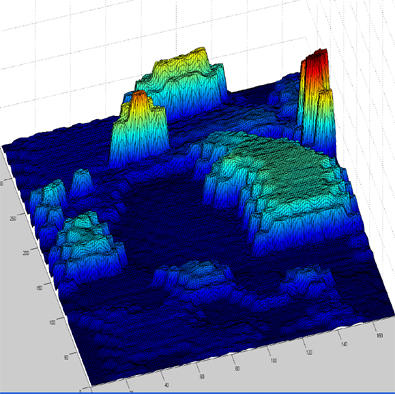
\includegraphics[width=1.5in]{3DMapDist.jpg}
	\caption{An example probability distribution map generated by a Bayesian model.}
	\label{3DMapDist}
	\end{minipage}
&
	\begin{minipage}{0.5\textwidth}
	\centering
	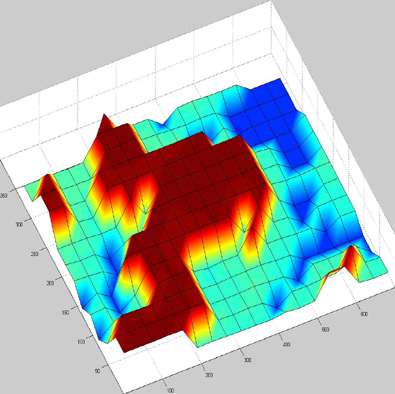
\includegraphics[width=1.5in]{3DMapDiff.jpg}
	\caption{An example task-difficulty map with three difficulty levels.}
	\label{3DMapDiff}
	\end{minipage}
\end{tabular}
\end{figure}


\begin{table}
\centering
		\begin{tabular}{|l|c|c|}
			\hline
				& \multirow{2}{*}{\textbf{Probability Distribution Map}} & \multirow{2}{*}{\textbf{Task-Difficulty Map}}  \\
				& & \\
			\hline
				\multirow{2}{*}{\textbf{Strategic}} & \textbf{TBMod} for map creation &  \\
				& \textbf{ParamMod} for info management & \\
			\hline
				\multirow{2}{*}{\textbf{Between-Episodes}} & \textbf{DistMod} for map update &  \textbf{DiffMod} for map update \\
				& and info management & and info management \\
			\hline
				\multirow{3}{*}{\textbf{Within-Episode}} & Extending algorithms to support & Extending algorithms to support\\
				& real-time feedback &  partial detection \\ \cline{2-3}
				& \multicolumn{2}{|c|}{\textbf{SlideMod} for info management} \\
			\hline
		\end{tabular}
	\caption{Components of proposed work}	
	\label{components}
\end{table}

%\begin{figure}
%\centering
%\begin{tabular}{cc}
%	\begin{minipage}{0.5\textwidth}
%	\centering
%	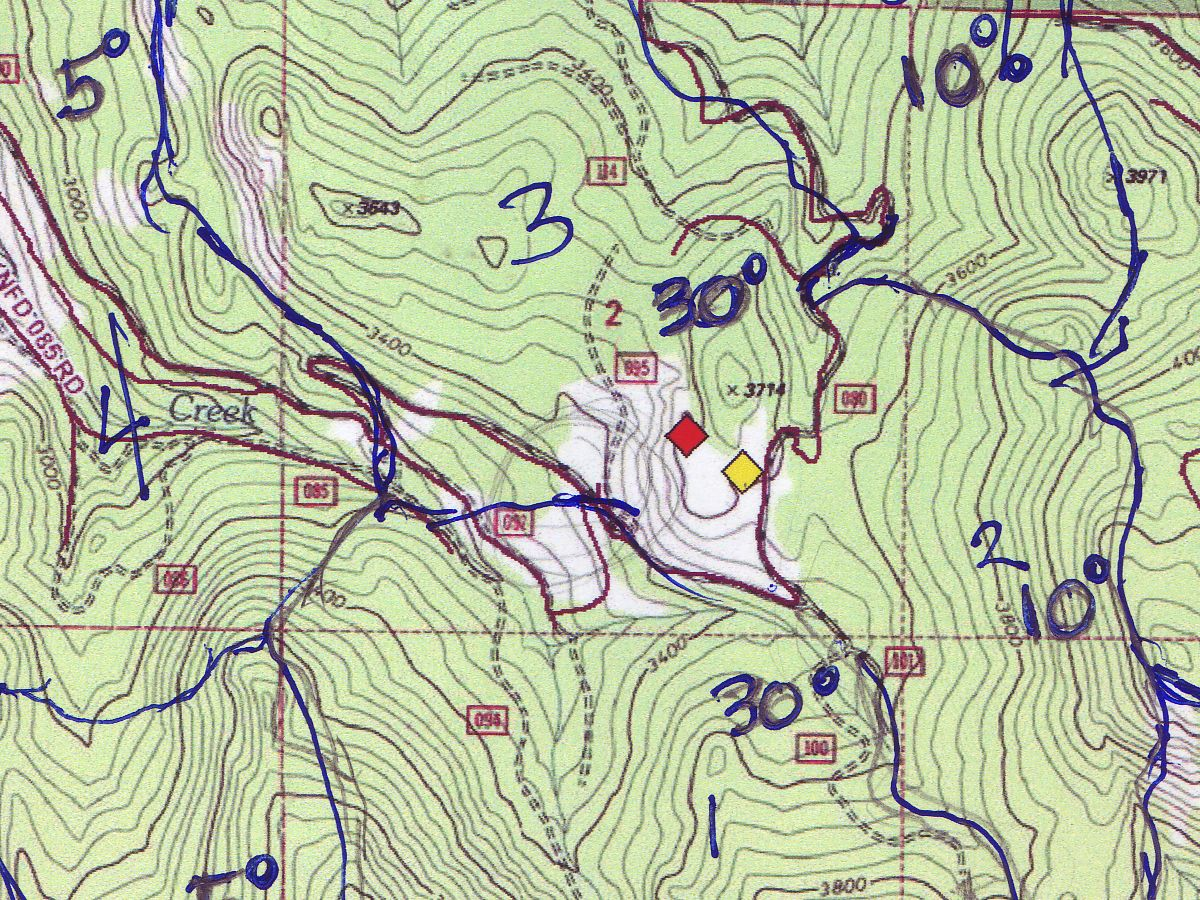
\includegraphics[width=2.0in]{RescuerMap.jpg}
%	\caption{A probability distribution map created by a real searchers in an exercise.}
%	\label{RescuerMap}
%	\end{minipage}
%&
%	\begin{minipage}{0.5\textwidth}
%	\centering
%	\includegraphics[width=1.5in]{3DMap.jpg}
%	\caption{A 3D probability distribution map generated by a Bayesian model.}
%	\label{3DMap}
%	\end{minipage}
%\end{tabular}
%\end{figure}

Table~\ref{components} lists the various components of our proposed work as they relate to these two map representations. At the strategic scale, we will develop a Bayesian model \textbf{TBMod} to systematically generate the probability distribution map. We will also build an information management tool, \textbf{ParamMod}, that lets the user manage ``user-friendly'' model parameters. Other members of our research group are working on building models to systematically generate the task-difficulty map (under various other names such as see-ability or visibility maps), therefore we do not include this component in the dissertation at the strategic scale. At the between-episodes scale, we will build a \textbf{DistMod} tool and a \textbf{DiffMod} tool that enable the user to modify the probability distribution map and the task-difficulty map respectively. At the within-episode scale, we will extend existing path-planning algorithms to support real-time feedback and partial detection. We will also build an information management tool, \textbf{SlideMod}, that lets the user prioritize search regions and manage the amount of autonomy desired.

Note that we have previously developed Intelligent Path Planning algorithms~\cite{Lin2009UAV} to generate UAV flight paths automatically with the objective to maximize the probability of finding the missing person based on the given probability distribution map.


%===================================================
\subsection{At the Strategic Scale}

At the strategic scale, a probability distribution map and a task-difficulty map can be created systematically. This dissertation will focus on developing information management tools for the probability distribution map. 

In work~\cite{Lin2010Bayesian} that will become on chapter in the dissertation, we established a Bayesian model (\textbf{TBMod}) that can generate the probability distribution map systematically using three types of terrain features (topography, vegetation, and elevation) and past human behavior data. Searchers first specify transitional probabilities (Beta distributions) between two terrain features as inputs. Then the model produces the prior/posterior~\cite{Russell2009Artificial} predictive probability distribution(s), which can be used to allocate resources and plan UAV paths. The management tool at this scale would allow the user to manage two types of information: \textit{model parameters} and \textit{dataset}.

The \textit{model parameters} should be limited to those that allow the user to easily infer the relationships between changes in the the parameter and changes in the probability distribution map. We represent the probability distribution map in discretized form using a hexagonal tessellation of the search region. We use Monte Carlo methods to encode changes in the map, so model parameters include transition probabilities (probability of a missing person moving from one hexagonal cell to a neighbor) and simulation parameters (for the MCMC algorithm). Transition probabilities are easily interpreted by search experts, but algorithm parameters are not.

After the searcher provides some initial lost person profile information (such as age, gender, etc.), the system will suggest transitional probability values based on statistics from past incidents~\cite{Koester2008Lost}. The searcher can use the suggested parameters or specify them manually using the proposed information management tool, \textbf{ParamMod}. Figure~\ref{Mockup1} shows a mock up screen of the \textbf{ParamMod} tool. A searcher can move two sliders to set the mean and standard deviation of a Beta distribution and see immediately how the shape of the Beta distribution would change respectively. We use mean and standard deviation parameters because they are easy to understand (in contrast to the $\alpha$ and $\beta$ parameters in the Beta distribution function). As the searcher changes the shape of each transitional probability distribution, the searcher will also see immediately how the changes affect the final 3D probability distribution map. This immediate visual feedback allows the user to understand causal effects and therefore helps the user form a mental model of the system that is similar to how the system truly works. Computationally, instant feedback requires that we perform matrix computations on the GPU using CUDA (Compute Unified Device Architecture) architecture. We have been collaborating with Mike Roscheck to implement this and will publish a paper on it.

\begin{figure}
\centering
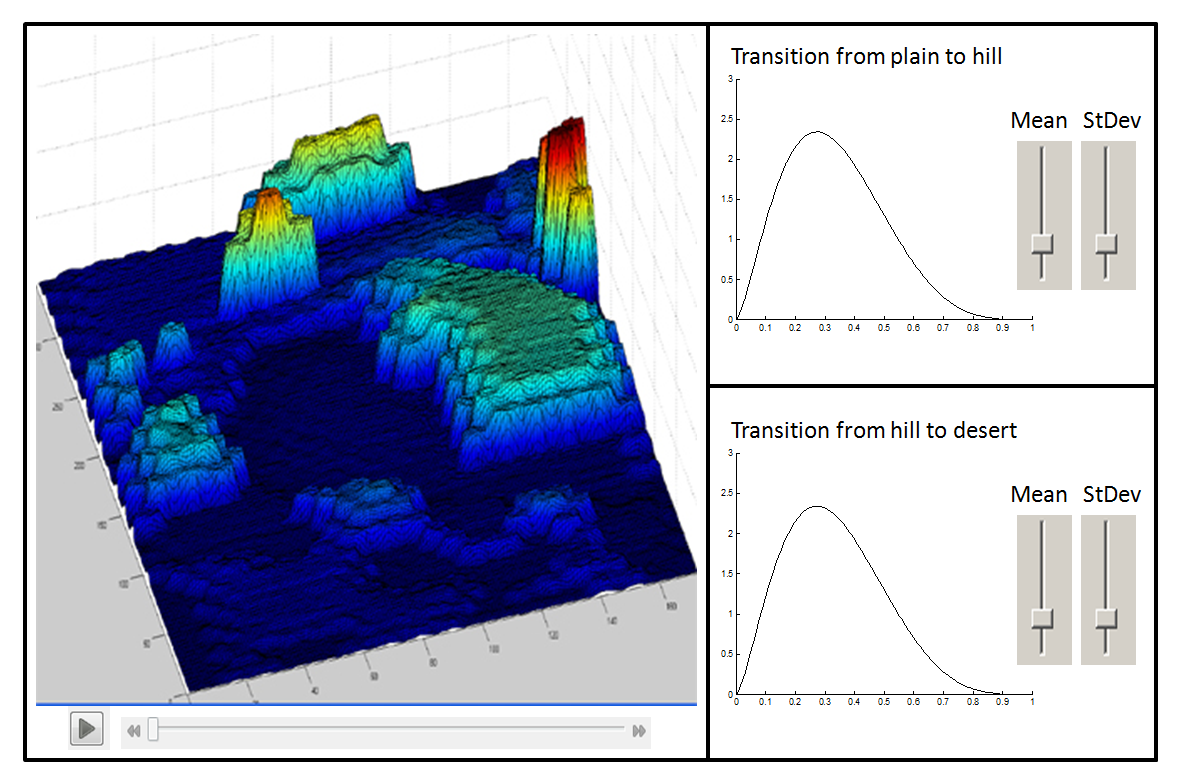
\includegraphics[width=3in]{Mockup1.png}
\caption{A mock up screen for the management tool interface at the general trend scale.}
\label{Mockup1}
\end{figure}

%The current Bayesian model uses external calls to MATLAB for large-size matrix multiplications and it takes roughly 4 seconds to multiple two 608 $\times$ 608 matrices. Since one matrix multiplication is needed for each time interval (1 minute), generating a predictive probability distribution for a 3-hour duration would require 180 matrix multiplications, which will take 12 minutes computation time. If after a user changes a model parameter, he/she has to wait 12 minutes to see how the parameter change affects the final product of the model, it is not very useful especially with respect to seeing the causal relationship. We propose to take advantage of powerful GPUs and use the CUDA (Compute Unified Device Architecture) parallel computation architecture developed by NVIDIA to speed up the matrix multiplications. Initial test runs of multiplying two 608 $\times$ 608 matrices on a GeForce GTX480 GPU took only 2 miliseconds. Such speed up enables the user to see immediately how parameter changes could affect the shape of the 3D probability distribution produced by the model. However, the immediate feedback is only avaible when computing the prior preditive probability (without using past human behavior data) because computing the posteriors of the transitional probabilities still takes 220 seconds when using the MCMC algorithm.

Although the term ``dataset'' can broadly include many sources of data, strategic data in WiSAR is available in only one form: GPS track logs of past human behavior. In this dissertation, we only let the searcher choose whether or not to use past human behavior data. If the user chooses not to use past human behavior dataset, the \textbf{TBMod} model will output the prior predictive distribution (prediction based only on the model parameters); otherwise, the model will output the posterior predictive distribution (prediction also based on past observations). Comparing the prior predictive to the posterior predictive distribution should allow the searcher to understand the causal relationship of how the decision affects the probability distribution map produced. We plan to use selected geocacher GPS track logs downloaded from Everytrail.com as the dataset. We will also create utility tools to process these GPS track logs, including automatically downloading and labeling related terrain features.

%Because intended destination and trail-following behaviors are important factors that can affect a lost person's behavior~\cite{Lin2010Bayesian}, we plan to include them in our \textbf{TBMod} model. Because trail data are not readily available directly from public resources, our utility tools will allow a user to trace trails from an overlaid satellite image of the region and add the topographical feature to the dataset. To add the intended destination feature, we include a prior node in our Bayesian network representing the probability of traveling to different directions with respect to how dispersed the direction is from the intended destination. This prior node will follow a categorical distribution, but the probability of each category is determined by a Gaussian distribution. A scaler parameter $s$ will be used to specify how the Gaussian distribution can be divided into different categories.

%The autonomy interface management tool should allow the searcher to first mark Point Last Seen and intended destination on the terrain map overlay, then specify lost person profile information such as age group and gender,  next choose whether to use past human behavior data, and finally choose whether to specify transitional probabilities manually.

%===================================================
\subsection{At the Between-Episodes Scale}

At the between-episodes scale, a searcher might have additional case-specific information (e.g, past experience, knowledge of the search area or weather conditions, or the profile of the missing person) and would like to modify the general plan produced at the strategic scale. Moreover, as search progresses, the search plan should change due to newly found evidence (or the lack of it) from either the ground searchers or previous UAV flights. We propose two management tools at this scale that allow the user to manage two types of information: \textit{areas of focus} and \textit{task difficulty}.

\begin{figure}
\centering
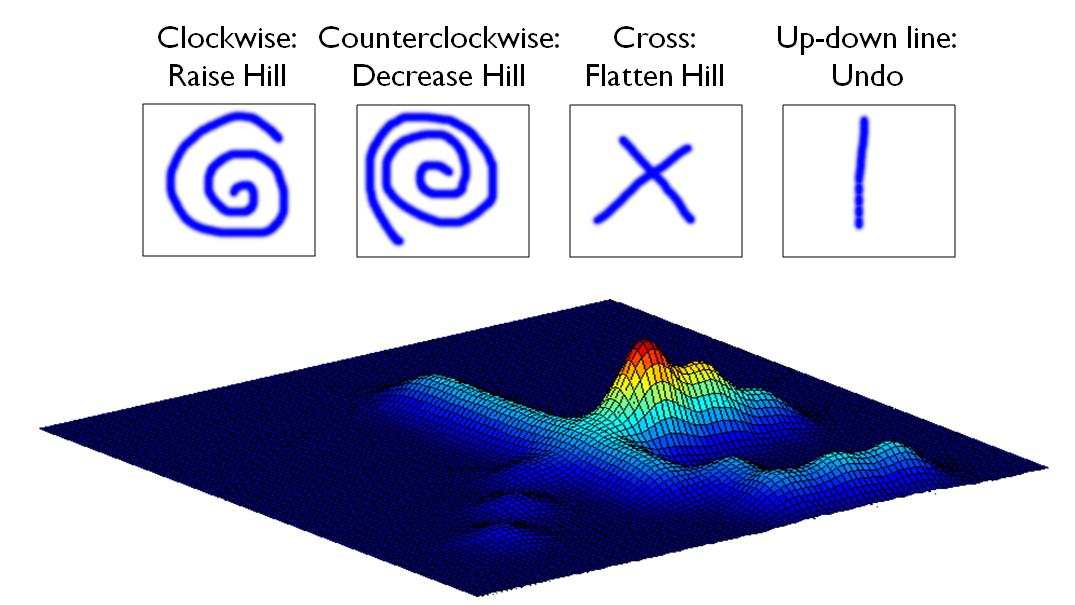
\includegraphics[width=3.5in]{Gestures.jpg}
\caption{Example gestures used to modify a probability distribution.}
\label{Gestures}
\end{figure}

The searchers can use simple mouse gestures (see Figure~\ref{Gestures} for examples) to specify \textit{areas of focus} that will modify the probability distribution map (created at the strategic scale) using the proposed \textbf{DistMod} tool. Users will modify the distribution by making mouse gestures over a 2D representation of the distribution map where colors are used to represent the probability density (e.g., red for high probability hills and blue for low probability plains/valleys). The searchers can switch to a 3D view (read-only) for a better view of the distribution surface. The modified probability distribution can be used later to prioritize tasks and plan UAV paths. By marking an area as a high priority area, the searchers can indirectly manipulate the UAV to search the area before other areas without the need to manually specify waypoints. We will use the feature set developed by Dean Rubine~\cite{Rubine1991Specifying} and use the k-Nearest Neighbor algorithm~\cite{Mitchell1997Machine} for gesture recognition.

The proposed \textbf{DiffMod} tool allows the searchers to create or modify the \textit{task-difficulty map}. A searcher can pick a difficulty level from a color pallet and then either select a difficult area (maybe due to dense vegetations or low visibility) with lasso capability or paint the area using scribbles. By marking an area as a difficult area, the user can indirectly tell the UAV to make multiple passes over these areas to search more thoroughly.

Both tools enable the searchers to add additional information to the probability distribution and task-difficulty maps, relying on UAV path-planning to use the information to search more efficiently.

%===================================================
\subsection{At the Within-Episode Scale}

When new evidence is gathered (from UAV aerial imagery or from ground searchers) while the UAV is flying, the search plan might need to be changed in real-time. At this within-episode scale, the information management tools \textbf{DistMod} and \textbf{DiffMod} previously proposed can be used to update the probability distribution and the task-difficulty maps. This provides flexibility in autonomy management. Additionally, we propose a management tool, \textbf{SlideMod}, that enables the user to prioritize search regions and manage the desired amount of the autonomous local search by changing the desired flight duration.

\begin{figure}
\centering
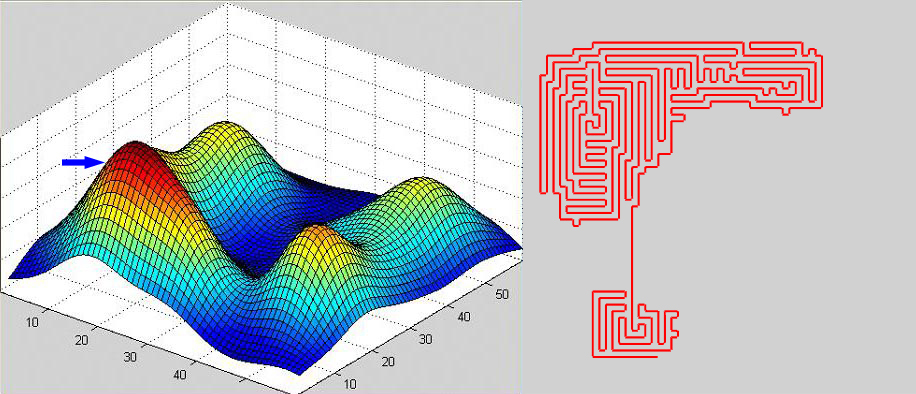
\includegraphics[width=3.5in]{ComplexMap.jpg}
\caption{Example UAV path generated for a complex multi-model distribution by a path planning algorithm. (The blue arrow indicates the starting point.)}
\label{path}
\end{figure}

Given a starting point, (optionally) an ending point, and a desired flight duration, our previously-developed Intelligent Path Planning algorithm (IPP)~\cite{Lin2009UAV} can generate flight paths that approximate the optimal path (see Figure~\ref{path} for an example) to maximize the probability of finding the missing person. The proposed \textbf{SlideMod} tool allows a searcher to specify a starting point and (optionally) an ending point on the terrain map overlay. Then, by moving a slider, the user can control how much flight time is granted, and the IPP algorithm generates UAV paths within the local region. Beginning from the ending point of the previous flight path segment, the searcher can plan the next path segment in the next search region. This way, the searcher can specify the order of different search regions and let the algorithm determine what paths the UAV should follow at each region. The searcher tells the UAV information about search constraints (search priorities) and at the same time, indirectly manages the local path planning based on his/her own judgment of how much the UAV can be trusted to cover a given area well. This management tool gives the user the flexibility of controlling the amount of autonomy desired without the burden of creating the entire flight path manually through waypoints. Figure~\ref{SlidingAutonomy} shows an example path depicting prioritized search regions and local paths.

\begin{figure}
\centering
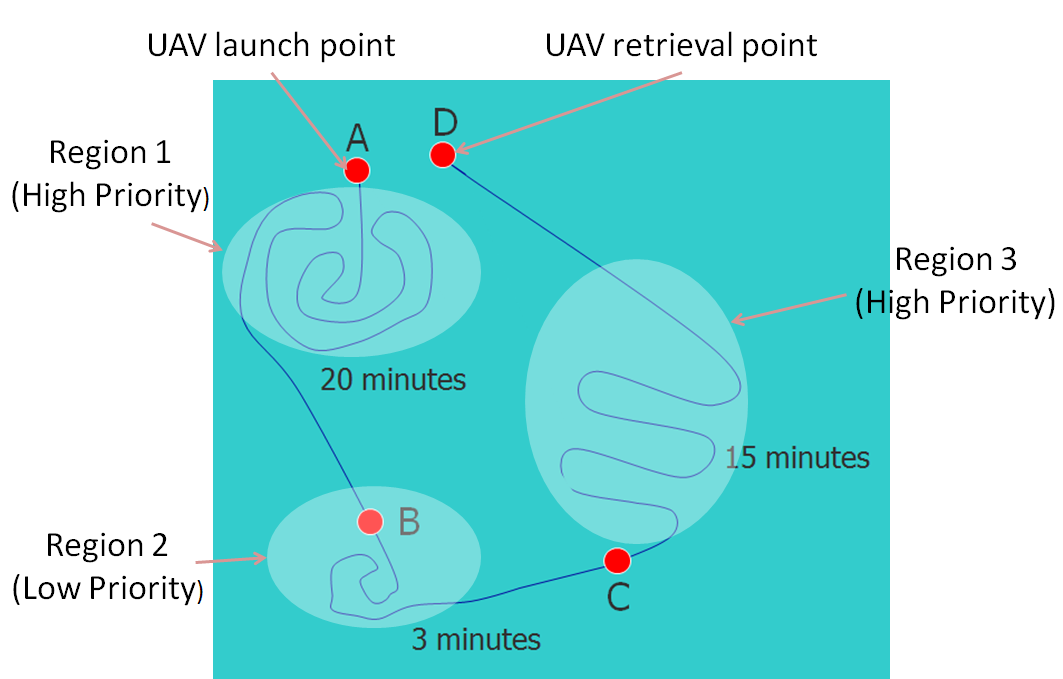
\includegraphics[width=3.5in]{SlidingAutonomyE.png}
%\caption[An example scenario of path planning using sliding autonomy]{An example scenario of path planning using sliding autonomy: The UAV starts at point A. The operator commands the UAV to plan a path for 20 minutes and specifies that the UAV should arrive at point B at the end of the flight. The operator then commands the UAV to plan another path from point B to point C for a 3-minute flight. Finally, the operator lets the UAV plan another path for 15 minutes but specifies that the UAV should arrive at point D at the end of the 15-minute flight for easy UAV retrieval.}
\caption[An example scenario of path planning using sliding autonomy]{An example scenario of path planning using sliding autonomy: The UAV is launched at point A. Because region 1 is a high priority area, the searcher lets the UAV search for 20 minutes before arriving at point B, resulting in a longer flight path. Region 2 has low priority, so the searcher only gives the UAV 3 minutes before sending the UAV to point C, resulting in a short flight path. Region 3 is a high priority area, so the searcher gives the UAV 15 minutes. But the UAV also needs to reach Point D, the UAV retrieval point, at the end of the allocated 15 minutes. A medium length flight path is generated to meet the requirements.}
\label{SlidingAutonomy}
\end{figure}

Ideally, as the user moves the slider in the \textbf{SlideMod} tool, the system will provide immediate visual feedback of what local path the system generates. This way, the searcher can easily infer the causal relationship between his/her actions (changes in flight duration) and the autonomous behaviors of the system (what path is generated). Presently, the IPP algorithm is slow and does not support real-time visual feedback. Also, the IPP algorithm assumes a 100\% probability of detection. In order to use the task-difficulty map the IPP algorithm needs to be extended to handle partial detection.

To speed up the path planning algorithms we plan to combine two techniques: 1) parallelize the seed paths generation; and 2) apply coarse-to-fine search along the added ``Global-Warming'' dimension~\cite{Lin2009UAV}. To support partial detection, we will modify the IPP algorithm to use the task-difficulty map. To validate the improved algorithm, we will follow the same validation method described in~\cite{Lin2009UAV}.


%=====================================================================================================
\section{Dissertation Chapters}

%===================================================
\subsection{Chapter Descriptions}

%===================================================
\subsection{Publications List}

We list all the citations for each chapter in the order in which they appear.

1. Jie Long, Cory Reimschussel, Ontario Britton, Anthony Hall, and Michael Jones. Performance Capture for Natural Tree Motions in the Wind. Motion in Games , MIG, 2010. 

2. Jie Long, Bryce Porter, Michael Jones. Motion Capture of Rope, not yet published.


%=====================================================================================================
\section{Contributions}


